\subsection{Artifact Requirements} \label{sec_artifact_requirements}

The primary objective of \citename{koks_convergence_2023}{author} research was to
determine the degree of convergence between \gls{ca} and NS Theory. To achieve this goal,
the research consited out of several key objectives.

Besides the a comprehensive literature analysis, an architectural design was created,
which was fully and solely based on \gls{ca} principles. The findings from the literature
review were incorporated into this design, which served as the basis for the subsequent
development of the research artifacts.

In the artifact development phase, two artifacts were constructed to facilitate the study
of the convergence between \gls{ca} and NS Theories. The first artifact was the Expander
Framework and Clean Architecture Expander. These components were designed and implemented
based on the \gls{ca} design principles. The Clean Architecture Expander enabled the
parameterized instantiation of software systems that adhere to the principles and design
of \gls{ca}, while the Expander Framework served as a supporting system. It was responsible for
loading and orchestrating dependencies, managing models, and executing the expander.

The second artifact was the Expanded Clean Architecture artifact. This artifact allowed
for the analysis of a RESTful API implementation and its alignment with \gls{ca}
principles and design, thereby providing a platform to evaluate the convergence of the two
theories in a practical context.

Finally, the analysis of combinatorics examined the artifacts for actual or potential
combinatorial effects. This analysis aimed to determine whether \gls{ca} and NS exhibit
convergence. The fundamental principles and architectural design of \gls{ca} were
considered throughout the analysis to ensure a comprehensive evaluation of the convergence
potential.

By pursuing these objectives, the research provides valuable insights into the interaction
between \gls{ca} and NS, particularly in terms of their potential convergence within the field
of software architecture.

This chapter outlines the construction of two artifacts. Both of these artifacts are
meticulously designed and developed in accordance with the design philosophy and
principles of \gls{ca} with strict adherence to the following requirements.

\subsubsection{Component Layer Naming Conventions} \label{appendix_component_naming_convention}

\textbf{[PROD]} is defined as \textit{The name of the product of the software.} \newline 
\textbf{[COMP]} is defined as \textit{The name of the Company that is considered the owner of the software. If
there is no company involved, this can be left blank.} \newline 
\textbf{[TECH]} is defined as \textit{The primary technology that is used by the component layer.} 

\begin{table}[H]
    \footnotesize
    \caption{Naming convention component layers}
    \begin{tabular}{ l l }
    \hline
    \textbf{Layer} & \textbf{Convention} \\ 
    \hline
    Domain & \textbf{Project}: [PROD].Domain \\ & \textbf{Package}: [COMP].[PROD].Domain \\
    Application & \textbf{Project}: [PROD].Application \\ & \textbf{Package}: [COMP].[PROD].Application \\
    Presentation & \textbf{Project}: [PROD].Presentation.[TECH] \\ & \textbf{Package}: [COMP].[PROD].Presentation.[TECH] \\
    Infrastructure & \textbf{Project}: [PROD].Infrastructure.[TECH] \\ & \textbf{Package}: [COMP].[PROD].Infrastructure.[TECH]
    \\ \hline
    \end{tabular}

\label{table:component_naming_convention}
\end{table}

\section{Element Naming Conventions} \label{appendix_element_naming_convention}

\textbf{[Verb]} is defined as \textit{The primary action that that class or interface is assosiated with.} \newline 
\textbf{[Noun]} is defined as \textit{The primary subject or object that that class or interface is assosiated with.} 

\begin{table}[H]
  \footnotesize
  \caption{Naming convention of recurring elements}
  \begin{tabular}{ p{0.16\linewidth} p{0.17\linewidth} p{0.09\linewidth} p{0.29\linewidth} }
  \hline
  \textbf{Layer} & \textbf{Element} & \textbf{Type} & \textbf{Convention} \\ \hline
  Presentation & Controller & class & [\textit{Noun}]Controller \\
  & ViewModel- Mapper & class & [\textit{Noun}]ViewModel- Mapper \\
  & Presenter & class & [\textit{Verb}][\textit{Noun}]Presenter \\
  & ViewModel & class & [\textit{Noun}]ViewModel \\

  Application & Boundary & class & [\textit{VerbNoun}]Boundary \\
  & Boundary  & interface & IBoundary \\
  & Gateway  & interface & I[\textit{Verb}]Gateway \\
  & Interactor  & interface & I[\textit{Verb}]Interactor \\
  & Interactor & class & [\textit{Verb}][\textit{Noun}]Interactor \\
  & Mapper  & interface & IMapper \\
  & RequestModel-Mapper & class & [\textit{Verb}][\textit{Noun}]Request-ModelMapper \\
  & Presenter  & interface & IPresenter \\
  & Validator  & interface & IValidator \\
  & Validator & class & [\textit{Verb}][\textit{Noun}]Validator \\
  
  Infrastructure & Gateway & class & [\textit{Noun}]Repository \\

  Domain & Data Entity & class & [\textit{Noun}] \\ \hline

  \end{tabular}
  
  \label{table_element_naming_convention}
\end{table}
\subsubsection{Component Architecture Requirements} \label{component_requirements}

The following requirements are applied to the component architecture of both the Generator
artifact and the Generated artifact.

\requirement{The component architecture}
\begin{enumerate}[label=\themycounter.\arabic*]
    \item The solution is organized into separate Visual Studio projects for the Domain,
    Application, Infrastructure, and Presentation layers of the component. A detailed
    description of these layers can be found in Section (((FIX FULLREF))).
    \item The Visual Studio projects representing the component layers comply with the naming
    conventions outlined in Appendix (((FIX FULLREF))).
    \item The dependencies between the component layers must follow an inward direction towards
    the higher-level components as illustrated in Figure \ref{fig_modulair_components}
    schematically, and cannot skip layers.
\end{enumerate}

\requirement{The technology}
\begin{enumerate}[label=\themycounter.\arabic*]
    \item The Domain and Application layers have no dependencies on infrastructure technologies, like web- or
    database technologies.
    \item The Presentation Layer relies on various infrastructure technologies for
    facilitating end-user interaction. Examples of such technologies include Command
    Line Interfaces (CLIs), RESTful APIs, and web-based solutions. Each dependency is
    isolated and managed in separate Visual Studio Projects to ensure the stability and
    evolvability of the system.
    \item The Infrastructure Layer may rely on other infrastructure components, such as
    databases or filesystems. Each infrastructure dependency is isolated and managed in
    separate Visual Studio Projects to promote stability and evolvability.
    \item All component Layers utilize the C\# programming language, explicitly targeting the
    .NET 7.0 framework.
    \item Reusing existing functionality or technology (packages) is permitted only when
    adhering to the \gls{lsp} and utilizing the open-source package manager,
    \gls{nuget}.
\end{enumerate}

\subsubsection{Software Architecture Requirements}\label{software_requirements}

Figure \ref{fig_design} illustrates the generic software architecture of the artifacts.
Each instantiated element adheres to the Element Naming Convention outlined in Appendix
(((FIX APPENDIX REF))). The following sections detail the requirements
specific to each element.

\begin{figure*}[ht!]
    \centering
    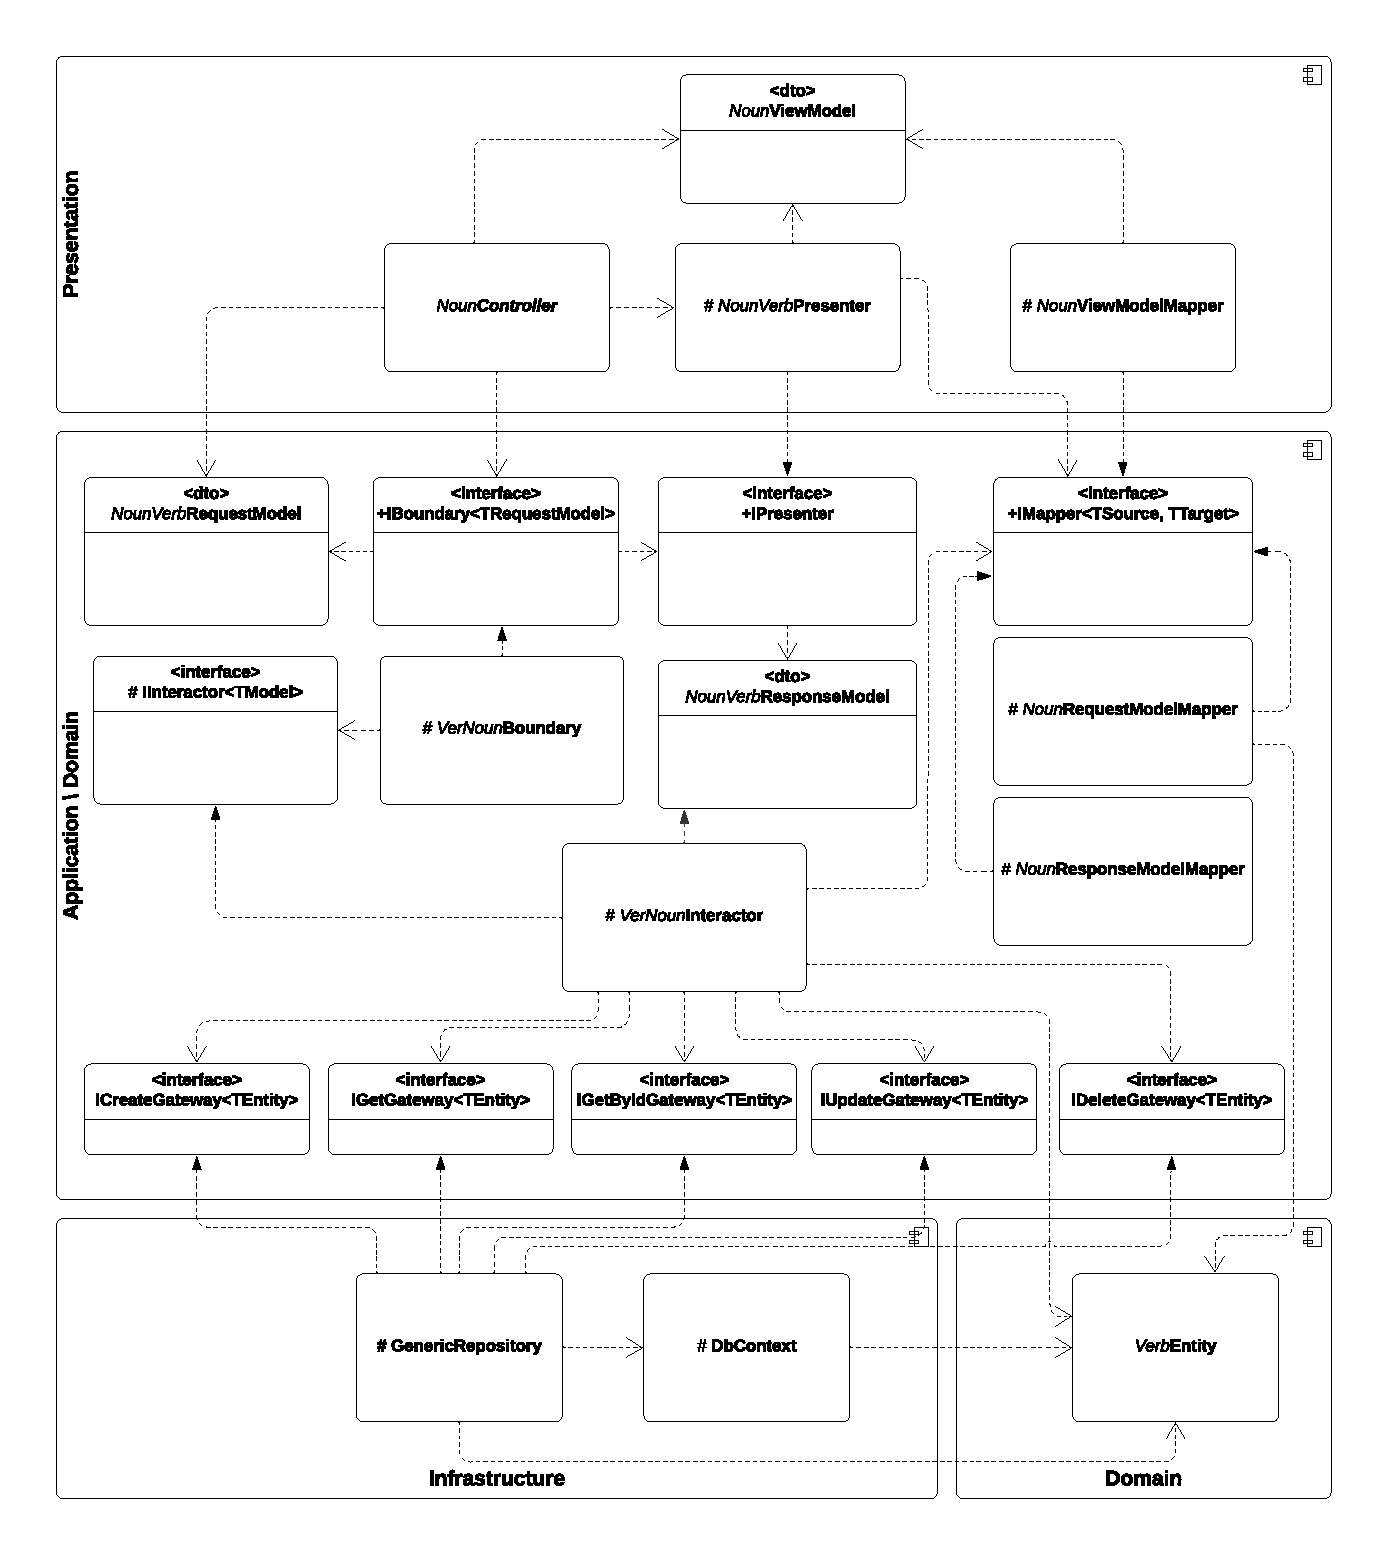
\includegraphics[width=\textwidth]{figures/generic_design.pdf}
    \caption[Generic architecture]{The Generic architecture of the artifacts}
    \label{fig_design}
\end{figure*}

The ViewModel consists of data attributes representing fields from the corresponding
Entity and may also contain information specific to the user interface. It is important to
note that the ViewModel has no external dependencies on other objects within the
architecture.

The Presenter is derived from the IPresenter interface and adheres to the specified
implementation, which is located in the Application layer. Its main responsibility is to
create the Controller's Response by instantiating the ViewModel, constructing the HTTP
Response message, or combining both as necessary. When needed, the Presenter utilizes the
IMapper interface without depending on specific implementations of IMapper. The Presenter
has an internal scope and cannot be instantiated outside the Presentation layer.

The ViewModelMapper, derived from the IMapper interface, follows the specified
implementation found in the Application layer. Its primary role is to map the necessary
data attributes from the ResponseModel to the ViewModel. The ViewModelMapper also has an
internal scope, ensuring it cannot be instantiated outside the Presentation layer.

The Controller is responsible for receiving external requests and forwarding them to the
appropriate Boundary within the Application layer. It relies on the IBoundary interface
without depending on specific implementations of this interface.

The IBoundary interface establishes the contract for its derived Boundary implementations,
and it has public scope within the system. Boundary implementations, derived from the
IBoundary interface, ensure separation between the internal aspects of the Application
Layer and the other layers. Each Boundary implementation handles a single task, executed
using the IInteractor interface. These implementations also have an internal scope and
cannot be instantiated outside the Application layer.

The IInteractor interface defines the contract for its derived Interactor implementations.
Like Boundary implementations, Interactors have an internal scope and are limited to the
Application layer. Interactor implementations execute single tasks or orchestrate a series
of tasks. Tasks dependent on infrastructure components, such as databases, are handled
through a Gateway. Additionally, Interactor implementations utilize the IMapper interface
to handle mapping between RequestModels, Entities, and ResponseModels.

The IMapper interface establishes the contract for Mapper implementations and has public
scope within the system. Derived from IMapper, the RequestModelMapper is responsible for
mapping the necessary data attributes from the RequestModel to an Entity. The
RequestModelMapper has internal scope and cannot be instantiated outside the Application
layer.

Similarly, the ResponseModelMapper is responsible for mapping data attributes from the
ResponseModel and follows the same implementation and scope restrictions as the
RequestModelMapper.

The IPresenter interface establishes the contract for Presenter implementations, typically
within the Presentation layer. It has public scope and ensures consistency in Presenter
behavior throughout the system.

The Gateway establishes the contract for interaction with infrastructure technologies such
as databases or filesystems. Each Gateway follows a specific naming convention, with
interfaces like ICreateGateway, IGetGateway, IGetByIdGateway, IUpdateGateway, and
IDeleteGateway representing different CRUD operations. Gateway implementations are derived
from these interfaces and are responsible for task-specific interactions with
infrastructure components. These implementations have internal scope and cannot be
instantiated outside their respective layers.

The ResponseModel consists of data attributes representing fields from the corresponding
Entity and may include output-specific data for the Interactor. The ResponseModel does not
depend on external objects within the architecture.

The RequestModel is similarly structured, consisting of data attributes from the
corresponding Entity and input-specific data for the Interactor. It, too, does not depend
on external objects within the architecture.

Data Entities represent corresponding data fields and do not rely on external objects.
They are only utilized by the Application layer.

The Gateway Implementation derives from the corresponding Gateway interface and adheres to
the specified implementation. It is responsible for handling tasks associated with its
infrastructure technology, such as interaction with a SQL database or filesystem. Gateway
Implementations have internal scope and cannot be instantiated outside their respective
layers.

Lastly, each architectural pattern adheres to at least one of the SOLID principles,
ensuring compliance and avoiding violations of these design principles.

\subsubsection{Expander Framework \& Clean Architecture Expander Requirements} \label{expander_framework_requirements}

In addition to the more generic requirements of previous sections, the following
requirements are specific for the Clean Architecture Expander \& Expander Framework artifact.

\requirement{The Expander Framework}
\begin{enumerate}[label=\themycounter.\arabic*]
    \item The Expander Framework enables interaction with the Clean Architecture Expander via a
    \gls{cli}. The \gls{cli} is implemented in the Presentation layer of the
    Expander Framework.
    \item The Expander Framework retrieves the model from an \gls{mssql} using the
    EntityFramework ORM technology. The EntityFramework technology is implemented in the
    Infrastructure layer of the Expander Framework.
    \item The Expander Framework loads and executes the configured Expanders. In the case of
    this research, only the Clean Architecture Expander is applied.
    \item The Expander Framework supports generic harvesting and injection, which can be
    used or extended by the Expanders using the \gls{ocp} principle.
    \item The Expander Framework supports generic template handling, which can be used or
    extended by the Expanders using the \gls{ocp} principle.
    \item The Expander framework adheres to this chapter's component and software Requirements
    specified in Sections \ref{component_requirements} and \ref{software_requirements}.
\end{enumerate}

\requirement{The Clean Architecture Expander}
\begin{enumerate}[label=\themycounter.\arabic*]
    \item The Clean Architecture Expander generates a C\# net7.0 RESTful service that provides an
    HTTP interface on top of the meta-model of the Expander Framework, allowing the basic
    \gls{crud} operations.
    \item The Clean Architecture Expander consists solely of an Application layer and reuses
    the Domain layer of the Expander Framework.
    \item The Clean Architecture Expander adheres to this chapter's component and software
    Requirements specified in Sections \ref{component_requirements} and
    \ref{software_requirements}.
\end{enumerate}

\subsubsection{Generated Artifact Requirements} \label{generated_artifact_requirements}


\requirement{The generated artifact}
\begin{enumerate}[label=\themycounter.\arabic*]
    \item The generated artifact adheres to this chapter's component and software
    requirements specified in Sections \ref{component_requirements} and
    \ref{software_requirements}.
\end{enumerate}
